\documentclass[a4paper,12pt]{article}

\title{Biology 30 IB \\ Cells, Chromosomes, \& DNA}
\author{Jad Chehimi}

% document setup
\renewcommand{\familydefault}{\sfdefault}
\linespread{1.25}
\usepackage[margin=1in]{geometry}
\usepackage{setspace}
\usepackage{enumitem}
\setlist{nosep}
\usepackage{amsmath}
\usepackage{color,soul}

% tools
\usepackage[hidelinks]{hyperref}
\usepackage{float}
%% images
\usepackage{graphicx}
\graphicspath{ {./images/} }
%% science
\usepackage{siunitx}

\begin{document}
\maketitle

% temp
\begin{center}
\Huge
Unfinished!
\normalsize
\end{center}
% temp

\tableofcontents

\pagebreak

\section{Terms}
\begin{itemize}
    \item{\textbf{Stomatic cells} are all cells in the body \hl{except sex cells} --- sperm and egg cells}
    \item{\textbf{Cell division} is done by Eukaryotic cells --- have a nucleus}
    \item{\textbf{Binary fission} is done by Prokaryotic cells --- have no nucleus, such as \hl{bacteria}}
\end{itemize}

\section{Cell Division}
\subsection{Purpose}
\begin{itemize}
    \item{Unicellular organisms (i.e. \hl{zygote}) $\longrightarrow$ Multicellular organisms}
    \item{Growth and maintenance of body cells --- \hl{replacement} of worn out cells}
\end{itemize}

\subsection{Chromosomes}
\begin{itemize}
    \item{
            Comprised of...
            \begin{itemize}
                \item{nucleic acids (DNA)}
                \item{proteins}
            \end{itemize}
        }
    \item{
            Either...
            \begin{itemize}
                \item{\textbf{Uncondensed} aka. \textbf{Chromatin} = long, thin strands. invisible to microscope}
                \item{\textbf{Condensed} = thick \& shortened. visible to microscope}
            \end{itemize}
        }
\end{itemize}

\subsection{Chromatid}
\begin{itemize}
    \item{The strand that makes up a normal chromosome}
    \item{
            In mitosis...
            \begin{itemize}
                \item{A chromosome duplicates into two \hl{identical} chromatids, joined together by a \textbf{centromere}, to form a \textbf{duplicated chromosome}}
                \item{These chromatids are referred as \textbf{sister chromatids} in this state}
                \item{Each chromatid of a duplicated chromosome goes to each of the two new cells}
            \end{itemize}
        }
\end{itemize}

\begin{figure}[H] 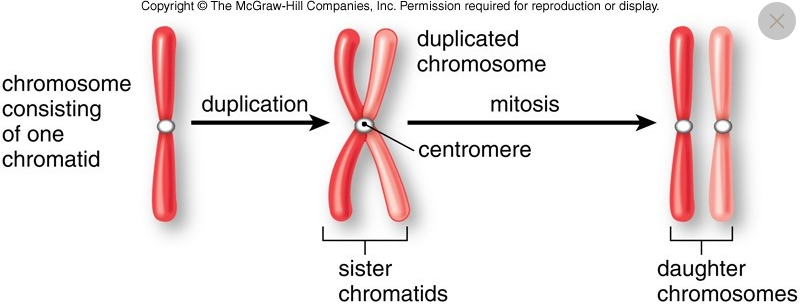
\includegraphics[width=\textwidth]{chromosome} \end{figure}

\section{Cell Cycle}
\begin{figure}[H] 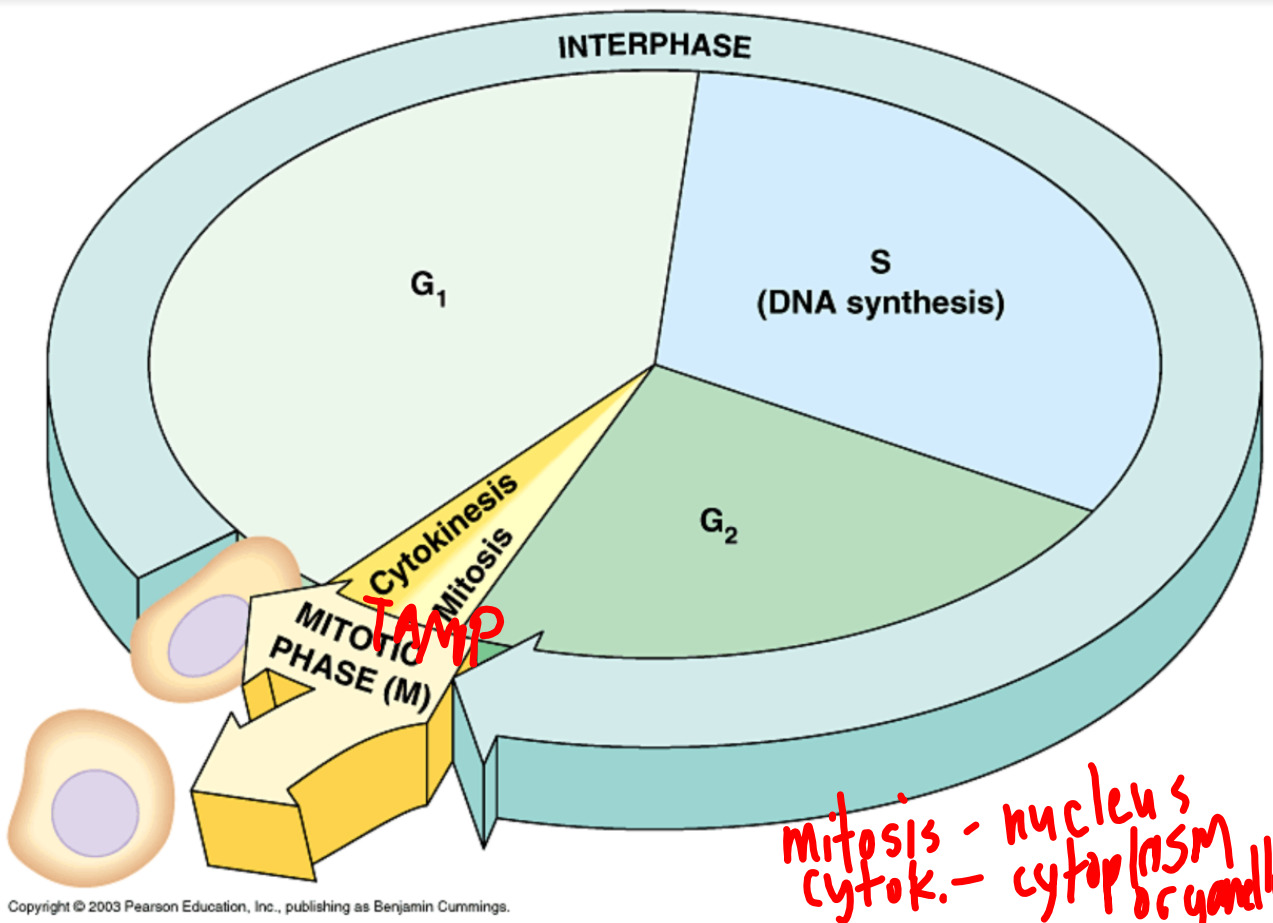
\includegraphics[width=\textwidth]{cellcycle} \end{figure}

A continuous cycle that involves all steps of a cell's life, especially cell division.

\subsection{Interphase}

\begin{itemize}
    \item{90\% of cell cycle}
    \item{All cell activity when not dividing}
\end{itemize}

\subsubsection{Gap 1 ($G_1$)}
\begin{itemize}
    \item{Cell growth and general function}
    \item{After cell division, cells may be smaller than their parent. Cell growth is needed}
\end{itemize}

\subsubsection{S Phase ($S$)}
\begin{itemize}
    \item{DNA is doubled}
    \item{Single(-chromatid) chromosome $\xrightarrow{\textrm{duplication}}$ double(-chromatid) chromosome}
\end{itemize}

\subsubsection{Gap 2 ($G_2$)}
\begin{itemize}
    \item{Organelles are doubled, and proteins for the new cell are produced}
\end{itemize}

\subsection{Mitotic Phase}\noindent

Occurs in stomatic cells.

Distribution of \hl{nucleus and its contents}.

\subsubsection{Prophase}
\begin{itemize}
    \item{Chromatin condense --- shorten \& thicken --- into chromosomes, becoming visible}
    \item{Nuclear membrane fades}
    \item{
            Animal cells only...
            \begin{itemize}
                \item{\textbf{Centrioles} move to opposite poles of cell. (N/S, E/W)}
                \item{Two centrioles are at each pole, total four, for each cell}
                \item{Centrioles deploy \textbf{spindle fibers}}
            \end{itemize}
        }
    \item{Without centrioles --- such as plant cells --- spindle fibers are still present and the cycle works the same}
\end{itemize}

\begin{figure}[H]
    \centering
    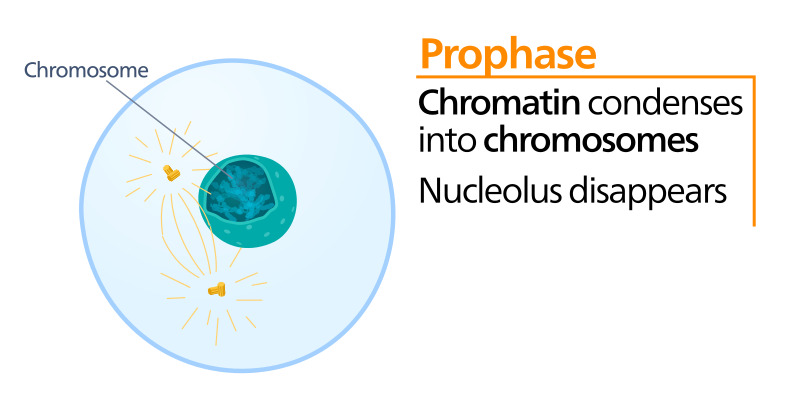
\includegraphics[width=0.5\textwidth]{prophase}
\end{figure}

\subsubsection{Metaphase}
\begin{itemize}
    \item{\textbf{Equatorial plate} = center of cell}
    \item{Sister chromatids move towards equatorial plate}
    \item{Chromosomes attach to spindle fibers}
\end{itemize}

\begin{figure}[H]
    \centering
    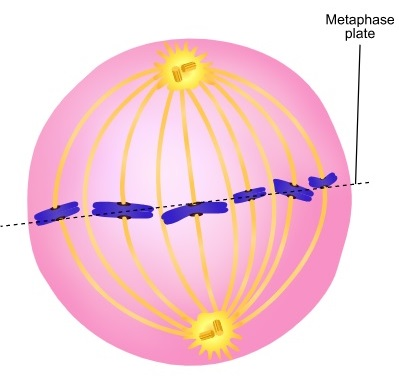
\includegraphics[width=0.5\textwidth]{metaphase}
\end{figure}

\pagebreak

\subsubsection{Anaphase}
\begin{itemize}
    \item{Centromeres divide}
    \item{(Now) chromatids move towards spindle fibers --- i.e. opposite poles of cell}
\end{itemize}

\begin{figure}[H]
    \centering
    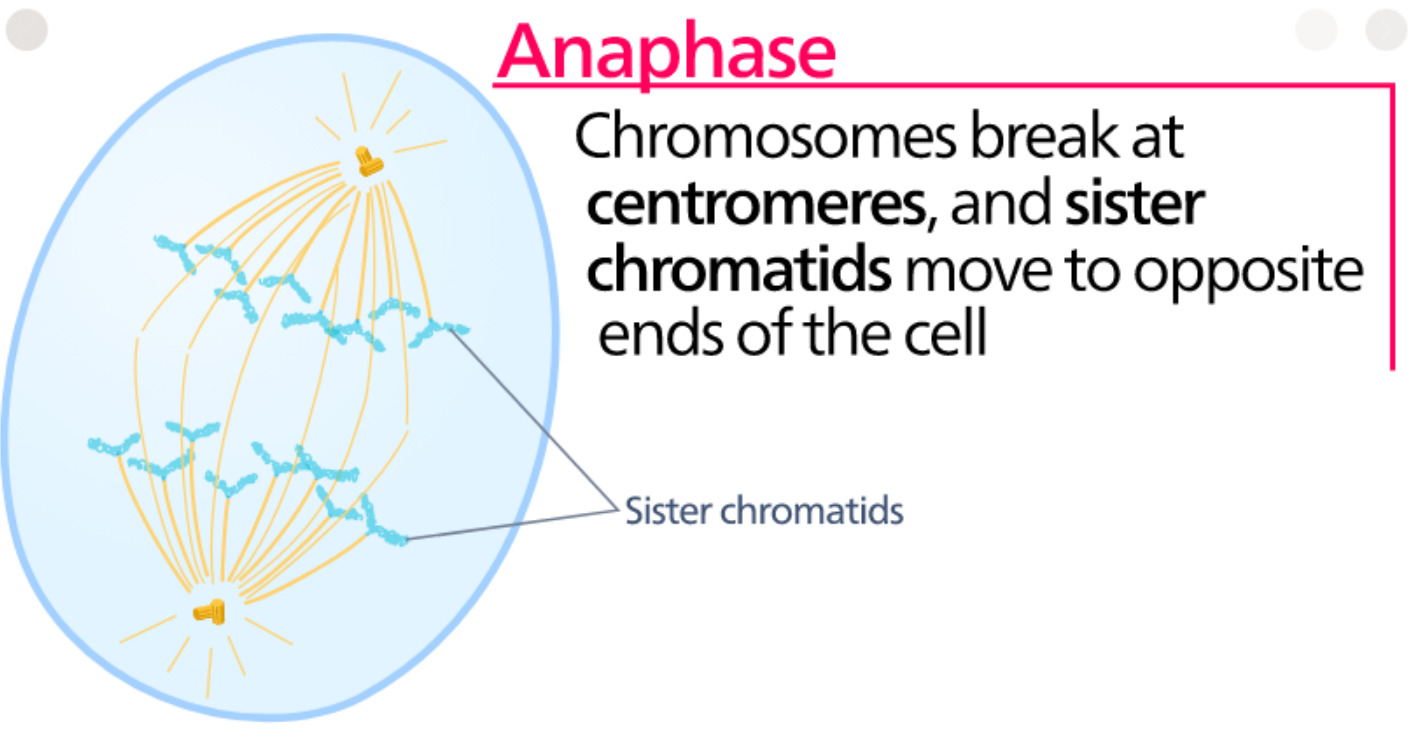
\includegraphics[width=0.75\textwidth]{anaphase}
\end{figure}

\subsubsection{Telophase}
\begin{itemize}
    \item{Spindle fibers dissolve}
    \item{Nuclear membrane forms around each mass of chromatin}
\end{itemize}

\subsubsection{Cytokinesis}
Technically occurs at the end of telophase.
\begin{itemize}
    \item{\hl{Division of cytoplasm} and \hl{distribution of organelles} to "daughter" cells}
    \item{Involves \textbf{cleavage}, pinching off in the center as the cytoplasm moves to opposite poles}
    \item{In plant cells only, a \textbf{cell plate} is distributed, which develops into a new cell wall}
\end{itemize}

\begin{figure}[H]
    \centering
    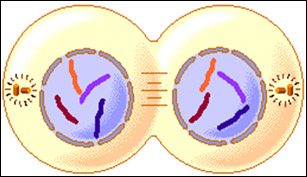
\includegraphics[width=0.75\textwidth]{telophase}
\end{figure}

\section{Cell Properties}

\subsection{Biological Clock}\noindent

Immature cells always have \hl{50 division}, regardless of...
\begin{itemize}
    \item{duration frozen}
    \item{stage/phase that cell division was suspended}
\end{itemize}

\subsection{Death \& Aging}\noindent

Cells may stop dividing due to...
\begin{itemize}
    \item{\textbf{Senescence} = aging, irreversible changes that eventually lead to death}
    \item{\textbf{Specialization} = the more \hl{specialized/differentiated} a cell is, the less likely it will undergo mitosis}
\end{itemize}

Cells that avoid aging are...
\begin{itemize}
    \item{\textbf{Spermatogonia} = sperm-producing cells, immature \& unspecialized}
    \item{Cancer cells of a tumor, which do not become specialized}
\end{itemize}

\section{Natural Cloning}
\begin{itemize}
    \item{Asexual/nonsexual reproduction}
    \item{Identical offspring from a single cell}
\end{itemize}

\subsection{Twins}
\begin{figure}[H]
    \centering
    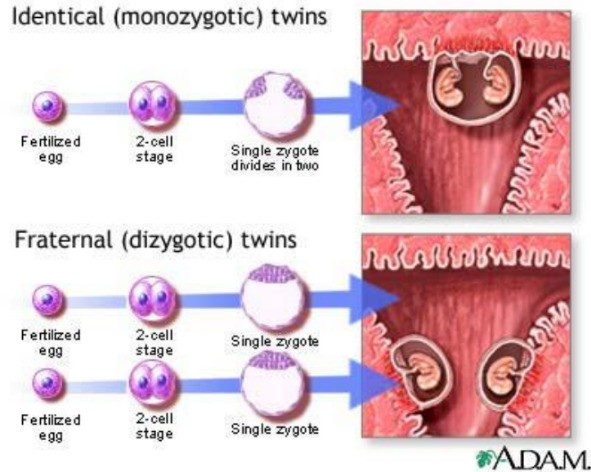
\includegraphics[width=0.9\textwidth]{twins}
\end{figure}

\subsection{Identical Twins}
\begin{itemize}
    \item{Originate from single egg cell}
    \item{During mitosis, \hl{one of the cells breaks free}; this cell forms a 2nd embryo}
    \item{If cell clusters remain separate, two babies with identical gene structures will develop}
    \item{Same gender, blood type, similar facial structure (nature vs. nurture)}
\end{itemize}

\subsection{Fraternal Twins}
\begin{itemize}
    \item{Two different eggs fertilized by different sperm cells}
    \item{Not to be confused with identical twins --- do not have identical genes}
\end{itemize}

\pagebreak

\section{Unnatural Cloning}

A \textbf{totipotent} nucleus is a nucleus that is able to bring a cell from \hl{egg to adult}.

\subsection{Plant Cloning}
\begin{itemize}
    \item{useful, since cloned plants have predictable characteristics}
    \item{requires \hl{delaying cell specialization}}
\end{itemize}

\subsection{Animal Cloning}
\begin{itemize}
    \item{With a micropipette, the nucleus is extracted from an unfertilized egg cell\\The cell is now \textbf{enucleated} (no nucleus)}
    \item{Remove nucleus from a cell of another frog}
    \item{Insert egg cell nucleus into said cell}
    \item{If cell is in \textbf{blastula} stage --- hollow ball of cells of an embryo, early embryo --- then the cells divide into an adult frog, a clone of the frog that donated the \hl{egg cell nucleus}}
    \item{If cell is past blastula --- such as the later \textbf{gastrula} stage --- the cells have \hl{already specialized}, so they do not divide, and the embryo dies}
\end{itemize}

\begin{figure}[H]
    \centering
    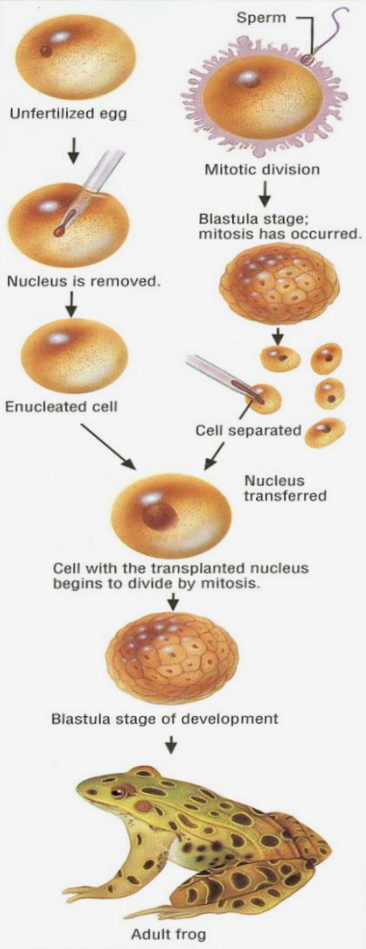
\includegraphics[width=0.3\textwidth]{clone}
\end{figure}

\subsubsection{Mammal Cloning}
\begin{itemize}
    \item{More difficult}
    \item{Cells tend to be \hl{more specialized}}
    \item{Nucleus transfer must be done before 8 cell stage of development}
    \item{Ensures nuclei are totipotent}
\end{itemize}

\begin{figure}[H]
    \centering
    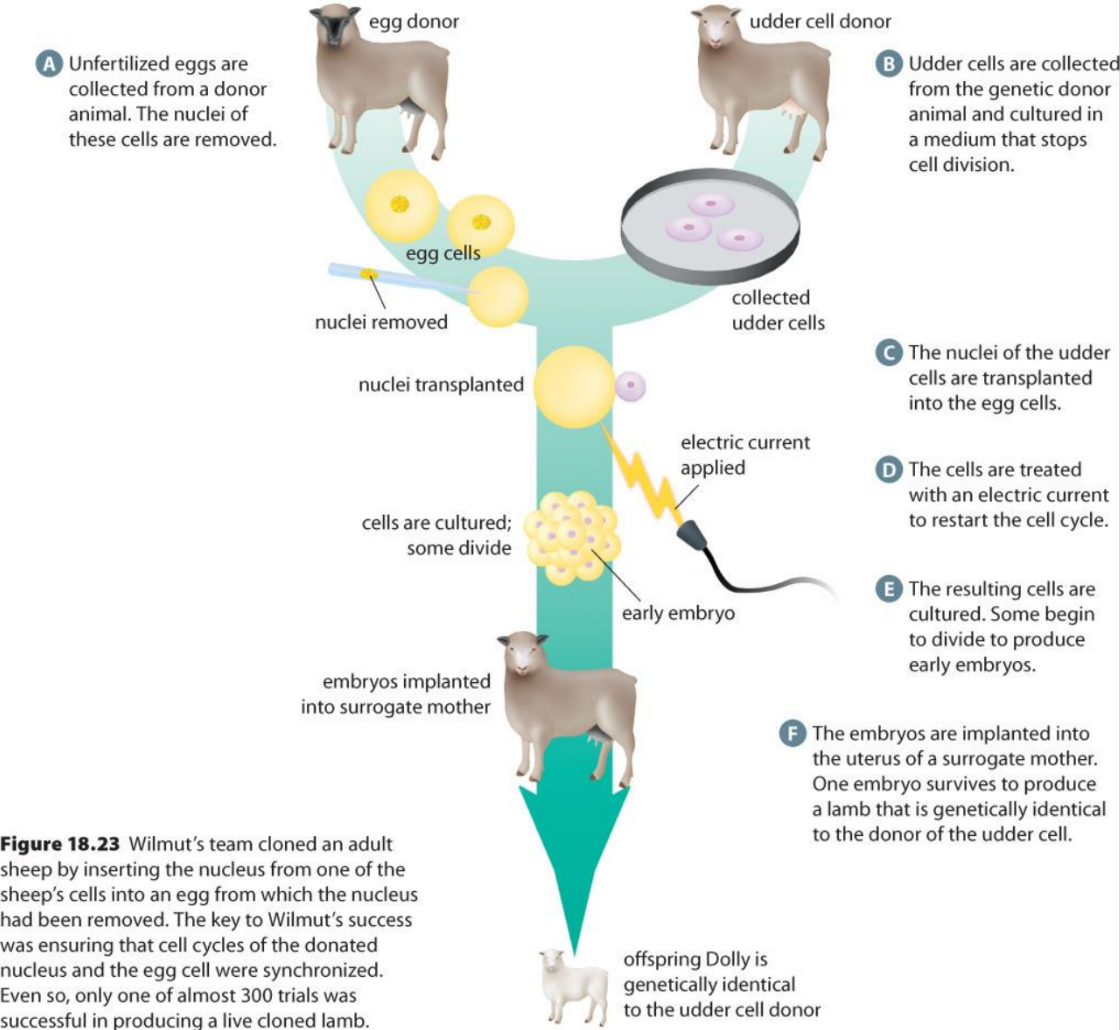
\includegraphics[width=\textwidth]{clone2}
\end{figure}

\pagebreak

\section{Cancer}
\begin{itemize}
    \item{Rapid, uncontrollable growth of cells}
    \item{Some are very slow, some pause and return after many years}
    \item{\hl{Reproduce without directions} from adjacent cells}
    \item{\hl{Cannot specialize} --- making them inefficient}
\end{itemize}

\subsection{Metastasis}
\begin{itemize}
    \item{Cancer cells can dislodge from a tumor and \hl{move to another area}}
    \item{Difficult to isolate source of cancer}
\end{itemize}

\subsection{Tumors}\noindent

A mass of cancerous cells within otherwise normal tissue.

\begin{itemize}
    \item{
            \textbf{Benign Tumor}

            \begin{itemize}
                \item{If cancerous cells remain at site}
                \item{Do not cause serious problems}
                \item{Can be removed by surgery}
            \end{itemize}
        }
    \item{
            \textbf{Malignant Tumor}

            \begin{itemize}
                \item{If cancerous cells metastasize --- dislodge \& travel --- and cause \hl{impairment of other organs}}
                \item{Unusual number of chromosomes}
            \end{itemize}
        }
\end{itemize}

\subsection{Causes}
\begin{itemize}
    \item{x-rays}
    \item{chemical poisons}
    \item{asbestos}
    \item{fungi}
    \item{oncoviruses}
    \item{environmental factors (nature, e.g. diet)}
    \item{age}
    \item{inherited mutations}
\end{itemize}

\subsection{Methods of Identification}
\begin{itemize}
    \item{x-rays}
    \item{cell biopsies}
    \item{infrared technology}
\end{itemize}

\section{Telomeres}
\begin{itemize}
    \item{Caps at the end of chromosomes}
    \item{\hl{Reduce in length every cell cycle/division}}
    \item{Clones --- like Dolly --- inherit their parents telomere length, \hl{shortening their life span} compared to non-clones} 
\end{itemize}

\begin{figure}[H]
    \centering
    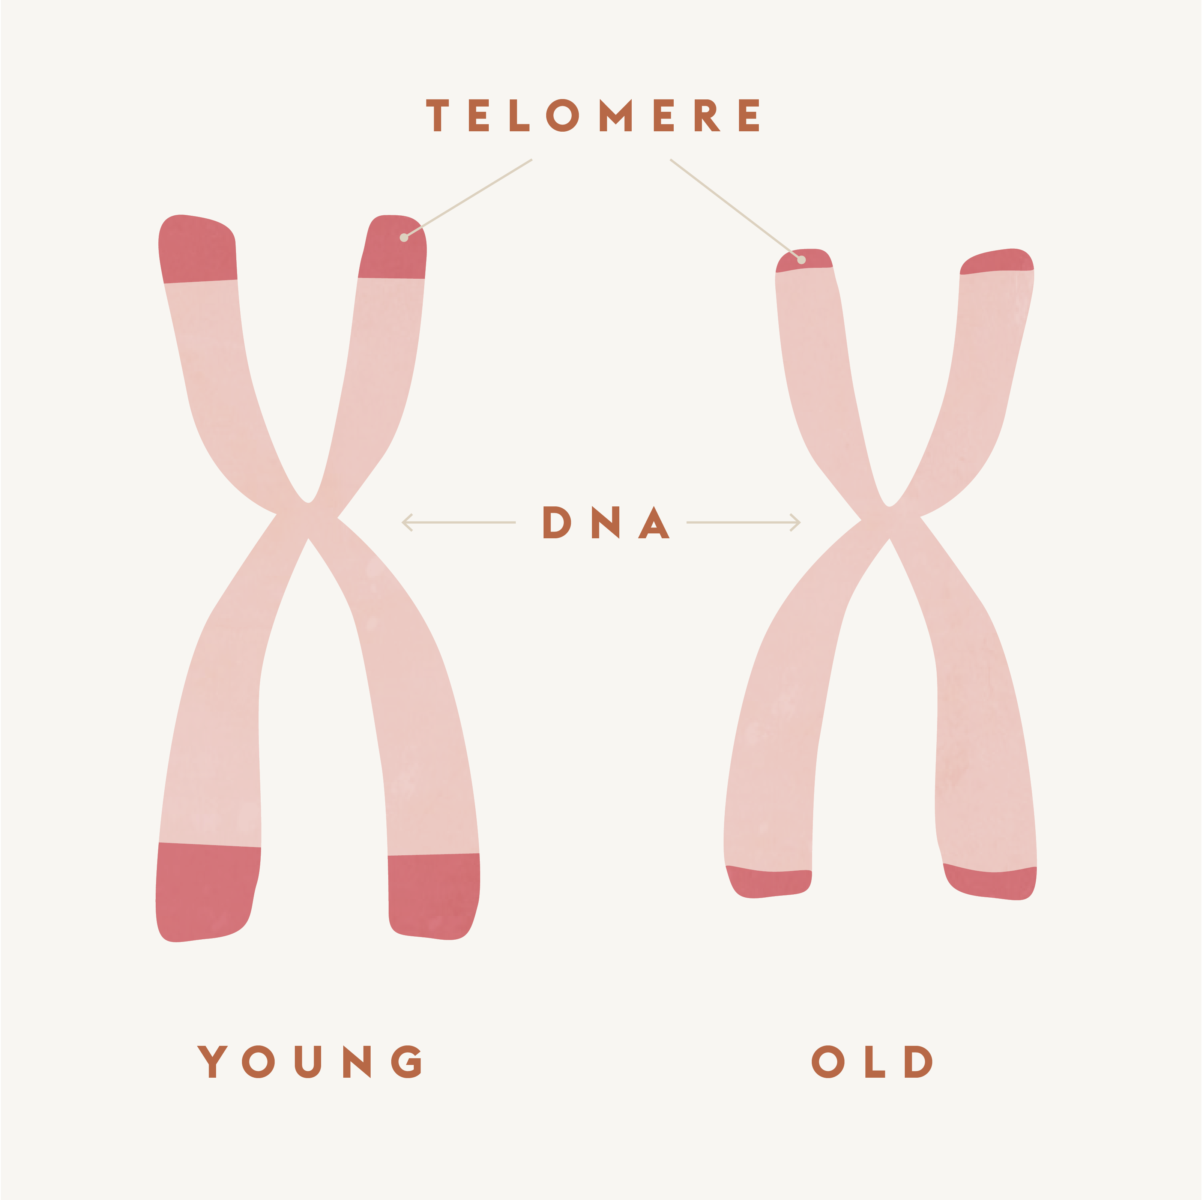
\includegraphics[width=0.50\textwidth]{telomere}
\end{figure}

\subsection{Telomerase}
\begin{itemize}
    \item{An enzyme that \hl{maintains telomere length}, slowing cell death}
    \item{Not present in most normal cells}
    \item{Reactivated in cancer cells, explaining their immortality}
\end{itemize}

\end{document}
